\documentclass[12pt]{article}
\usepackage[a4paper, total={7.5in, 10.5in}]{geometry}
%\usepackage{array}
\usepackage{graphicx, subfig, wrapfig, fancyhdr, lastpage, multicol ,color,arydshln,makecell,chemfig}
\usepackage[most]{tcolorbox}
\newcommand\headerMe[2]{\noindent{}#1\hfill#2}
\usepackage[mathscr]{euscript}
\usepackage{tabularray}

\setlength{\columnseprule}{1pt}
\def\columnseprulecolor{\color{blue}}


\pagestyle{fancy}
\fancyhf{}

\cfoot{\vspace{-1cm} \em{Page \thepage \hspace{1pt} / 4}}


\newtcolorbox{Box2}[2][
enhanced, 
    breakable,
]{
                lower separated=false,
                colback=white,
colframe=white!20!black,fonttitle=\bfseries,
colbacktitle=white!30!gray,
coltitle=black,
enhanced,
attach boxed title to top left={yshift=-0.1in,xshift=0.15in},
title=#2,#1
}
%    \vspace{.2cm}



\begin{document}

\headerMe{Royaume du Maroc}{année scolaire \emph{2023-2024}}\\
\headerMe{Ministère de l'Éducation nationale, }{  }\\
\headerMe{du Préscolaire et des Sports}{Établissement : \emph{Lycée SKHOR qualifiant}}\\
\vspace{-1cm}
\begin{center}
	Devoir Surveillé  N°2 - S2 \\

	2ème année baccalauréat Sciences Mathématiques\\
	%Durée 2h00
	%    \vspace{.2cm}
	\hrulefill
  \Large{--Chimie (7pts)--}
	\hrulefill\\

	% \emph{Les  parties sont indépendantes}
	%\emph{Les deux parties sont indépendantes}

	\vspace{-.2cm}
\end{center}
%end Headerss------------------------
%__________________Chimie ______________________-
%%%%%%%+_+_+_+_+_+_+_+_+_Partie1
\begin{Box2}{Etude de la pile Cuivre-Aluminium}


	\begin{wrapfigure}[21]{r}{0.44\textwidth}
		\begin{center}
			%\vspace{-2cm}
			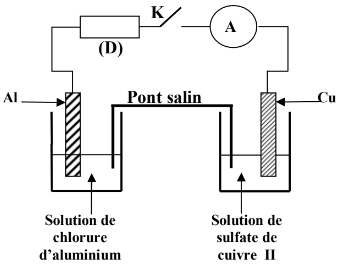
\includegraphics[width=0.4\textwidth]{./img/pile00.png}
			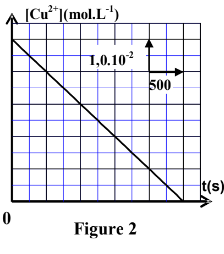
\includegraphics[width=0.3\textwidth]{./img/pile01.png}
		\end{center}
	\end{wrapfigure}



	\emph{ \textbf{ On avait découvert la pile qui met en œuvre les couples de type " Ion métal/Métal" à une
			époque où l’évolution du télégraphe nécessitait un besoin de sources de courant électrique
			continu. }}
	L’objectif de cette partie est l’étude de la pile Cuivre-Aluminium \dots
	\textbf{Données :}
	\begin{itemize}
		\item Constante de Faraday : $F = 96500 C/mol$
		\item Masse molaire atomique de l’élément aluminium: $M = 27g/mol$
		\item Constante d’équilibre associée à l’équation de la réaction entre le métal cuivre et les ions aluminium :
      $ 3Cu_{(s)} + 2Al^{3+}_{(aq)} \rightleftharpoons 3Cu^{2+}_{(aq)} + 2Al_{(s)}$ est $K = 10^{-20}$
	\end{itemize}

  On réalise la pile Cuivre - Aluminium
en reliant deux demi - piles par un pont
  salin de chlorure d’ammonium  $(NH_4^+ + Cl^-)$

  La première demi- pile est constituée
d’une lame de cuivre partiellement immergée
  dans une solution aqueuse de sulfate de cuivre II $(Cu^{2+} + SO_4^{2-})$

  de concentration $C_0$ et de volume $V = 50 mL$.
La deuxième demi-pile est constituée d’une
lame d’aluminium partiellement immergée
  dans une solution aqueuse de chlorure d’aluminium $(Al^{3+}$+$3Cl^-)$

  de même
concentration $C_0$ et de même volume $V$.
On branche entre les pôles de la pile un conducteur Ohmique (D), un ampèremètre et un
interrupteur K (figure1).

A l’instant t=0 on ferme le circuit , un courant électrique
d’intensité constante I circule alors dans le circuit .

La courbe de la figure2 représente la variation de
  la concentration $[Cu^{2+}]$ des ions cuivre II existant
dans la première demi- pile en fonction du temps .

	\begin{tabular}{c|l}
		0,5 & \makecell[l]{\textbf{1.1. }En utilisant le critère d’évolution spontanée, déterminer
le sens d’évolution du système\\chimique constituant la pile . }                                    \\

		0,5  & \makecell[l]{\textbf{1.2. }Donner la représentation conventionnelle de
la pile étudiée. }\\

    0,5 & \makecell[l]{\textbf{2.1} Exprimer la concentration $[Cu^{2+}]$ à un instant t en
fonction de $t$ , $C_0$ , $I$ , $V$ et $F$. }\\

		0,5 & \makecell[l]{\textbf{2.2. }En déduire la valeur de l’intensité I du courant électrique qui passe dans le circuit . } \\

		2  & \makecell[l]{\textbf{3. }La pile est entièrement usée à une date $t_c$ .Déterminer, en fonction de $t_c$ , $F$ , $I$ et $M$,\\la
    variation $\Delta{m}$ de la masse de la lame d’aluminium lorsque la pile est entièrement usée.
    \\Calculer $\Delta{m}$ . }                                    \\

	\end{tabular}
\end{Box2}

\begin{Box2}{Etude de la pile Cuivre-Aluminium}
  On étudie la pile Cadmium – Argent qui fait intervenir les deux couples ox/red : $Ag_{(aq)^+ / Ag_{(s)}}$ et $Cd_{(aq)^{2+} / Cd_{(s)}}$
	\textbf{Données :}
	\begin{itemize}
		\item Constante de Faraday : $F = 96500 C/mol$
    \item La partie immergée de l’électrode consommable est en excès.
    \item Masse molaire atomique de l’élément Cadmium: $M(Cd) = 112,4 g/mol$
		\item Constante d’équilibre associée à l’équation de la réaction entre le métal cuivre et les ions aluminium :
      $ 2Ag^+_{(aq)} + Cd_{(s)} \rightleftharpoons 2Ag + Cd^{2+}$ est $K = 5.10^{40}$
	\end{itemize}
On réalise cette pile, en plongeant une lame d’argent dans un bécher contenant un volume

$V= 250mL$ d’une solution aqueuse de nitrate d’argent $(Ag^+_{(aq)}) + NO^-_{3(aq)}$ de concentration molaire initiale 
  $C_1 = [Ag^+_{(aq)}]_i = 0,400 mol/L$, et une lame de cadmium dans un autre bécher contenant un volume

$V = 250mL$  d’une solution aqueuse de nitrate de cadmium $(Cd^{2+} + 2.NO^-_{3(aq)})$ de concentration molaire

  initiale $C_2 = [Cd^{2+}]_i = 0,200 mol/L$ .On relie ensuite les deux solutions par un pont salin.

On branche entre les électrodes de la pile un conducteur ohmique monté en série avec un ampèremètre
et un interrupteur.

\begin{enumerate}
  \item Choisir la proposition juste parmi les affirmations suivantes :\dots(0,5pt)
    \begin{enumerate}
      \item Les transformations se produisant dans les piles sont forcées.
      \item Le pôle positif de la pile est l’électrode d’argent.
      \item Le sens spontané d’évolution du système chimique constituant la pile est le sens (2) de l’équation de la réaction.
      \item L’oxydation se produit au niveau de la cathode.
    \end{enumerate}
  \item On ferme le circuit à un instant choisi comme origine des dates
    $(t=0)$. Un courant, d’intensité $I=215mA$ .considérée constante, circule alors dans le circuit
    \begin{enumerate}
      \item[1.] Exprimer, à un instant $t$, le quotient de réaction $Q_r$ en fonction de l’avancement $x$ de la réaction\dots(0,5)
      \item[2.] Calculer $Q_r$ à l’instant $t=10h$\dots(1pt)
      \item[3.] Calculer $|{\Delta{m}}|$, la variation de la masse de l’électrode de cadmium entre l’instant $t = 0$et l’instant où la pile est usée \dots{(1pt)}

    \end{enumerate}
\end{enumerate}
\end{Box2}


\begin{center}
	\hrulefill
  \Large{--Mécanique (13pts)--}
	\hrulefill\\

\end{center}
\vspace{0.7cm}

\begin{Box2}{PARTIE I : SAUT DU PLONGEUR DANS L’AIR }




	\emph{Dans tout l’exercice le mouvement du centre d’inertie du plongeur de masse m = 70kg est étudié dans le
repère d’axes (Ox, Oy) . }

  On prendra pour la valeur du champ de pesanteur $g = 9, 81m.s^{-2}$
et on considèrera que le référentiel terrestre
est galiléen. On note $y_0$ l’ordonnée du centre d’inertie du plongeur à l’instant où il quitte le tremplin et $v_0$ sa
  vitesse initiale formant un angle $\alpha = 30^{\circ}$ avec l’horizontale.
On donne $v_0 = 5m/s$
et $y_0 = 4,0m$ .

	\begin{enumerate}
    \item Établir les équations horaires du mouvement du centre d’inertie G du plongeur\dots(1pt)
    \item Déterminer l’équation cartésienne de la trajectoire. En déduire sa nature.\dots(1pt)
    \item Déterminer les coordonnées du centre d’inertie G du plongeur lorsque ses mains touchent l’eau on donne
      que $y_1 = 1m$ (voir figure 1)\dots(1pt)
    \item Calculer la durée tp du plongeon\dots(1pt)
    \item Déterminer la hauteur maximale H atteinte par le plongeur au cours du plongeon\dots(1pt)
	\end{enumerate}
	\begin{center}
		%	  \vspace{-2cm}
		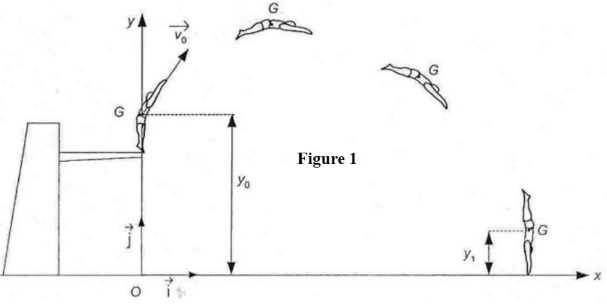
\includegraphics[width=0.49\textwidth]{./img/plangeur00.png}
		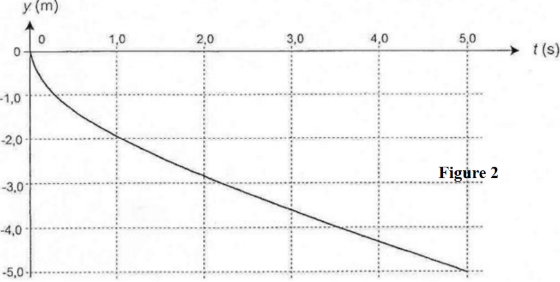
\includegraphics[width=0.49\textwidth]{./img/plangeur01.png}
	\end{center}

\section*{PARTIE II: MOUVEMENT DU PLONGEUR DANS L’EAU}
Le mouvement du centre d’inertie G du plongeur est considéré comme vertical dans cette partie. La profondeur du bassin dans lequel évolue le plongeur est de $5,0 m$.

	\begin{enumerate}
		\item La figure 2 résulte d’une simulation et représente l’évolution de l’altitude y du centre d’inertie du plongeur
au cours du temps.
On précise que l’on a pris comme origine des dates l’instant où le centre d’inertie atteint la surface de
l’eau.

      Pour pouvoir remonter, le plongeur doit redresser son buste.
On estime que le plongeur agit activement pour amorcer sa remontée 1,0 s après que son centre d’inertie
a atteint la surface de l’eau.

      De plus, on considère que le centre d’inertie du plongeur se situe toujours à 1,0 m de ses mains tendues.
Au moment où il amorce sa remontée, les mains du plongeur ont-elles atteint le fond du bassin ? Justifier
      la réponse\dots(1pt)
    \item On se propose de modéliser le mouvement du centre d’inertie du plongeur dans l’eau s’il n’amorçait pas
de remontée.
On note $V$ le volume du plongeur et $\rho$ la masse volumique de l’eau de la piscine.
Le plongeur est soumis, entre autres, à une force de frottement fluide dont le sens est opposé celui du
vecteur vitesse et dont la valeur peut être modélisée par $f = k.v^2_y$ où k comme une constante. et $v_y$ est la
composante du vecteur vitesse du centre d’inertie sur l’axe vertical orienté vers le haut
\begin{enumerate}
  \item[1]  Nommer les forces qui s’exercent sur le plongeur lors de ce mouvement. Les
    représenter, sans souci d’échelle, en son centre d’inertie G\dots(1pt)

  \item[2] En appliquant la deuxième loi de Newton, montrer que l’équation différentielle
    qui régit le mouvement du centre d’inertie du plongeur est donnée par :\dots(1pt)
    $$\frac{m}{k}.\frac{dv_y}{dt} - v^2_y = \frac{g}{k}.(\rho.V - m)$$

  \item[3] En déduire, en la justifiant, l’expression en régime permanent de la valeur $v_p$ du vecteur vitesse\dots(1pt)
  \item[4] Calculer $v_p$ . On prendra  $\rho =  10^3.kg.m^3$ ;$V = 6,5.10^{-2}.m^3$ et $k = 150 Kg/m$\dots(1pt)
  \item[5] En exploitant la courbe , dire si le plongeur a atteint le régime permanent avant que ses mains ne
    touchent le fond\dots(1pt)
\end{enumerate}
\item La méthode de résolution numérique d’Euler, permet de calculer de façon approchée la valeur algébrique
de la vitesse instantanée verticale $v_y$ à différentes dates. On note :
\begin{itemize}
  \item $v_y(t_n)$ la valeur algébrique de la vitesse à l’instant de date $t_n$.
  \item la valeur algébrique $v_y(t_{n+1})$ à la date $t_{n + 1} = t_n + \Delta{t}$ est calculée en utilisant la relation suivante:
    $v_y(t_{n+1}) = v_y(t_n) + a_y(t_n).\Delta{t}$
    
    où $a_y$ est la composante de l’accélération selon l’axe (Oy) et $\Delta{t}$ est le pas de calcul.

Compte tenu des valeurs numériques , l’équation différentielle obtenue précédemment permet d’obtenir la
    relation suivante : $$a_y(t) = 2,14.v^2_y(t) - 0,7$$ $\Delta{t} = 1,2.10^{-2}s$
\end{itemize}
      En utilisant la relation (1) pour le calcul de $v_y(t_{n+1})$ et la relation (2) pour celui de $a_y(t_n)$, compléter
      avec des valeurs numériques le tableau suivant :\dots(2pt)

\begin{center}
\begin{tabular}{ c c c }
  Date en s & $v_y$ en $m/s$ & $a_y$ en $m.s^{-2}$ \\ 
  $t_n = 0,144s$ & $v_y(t_n) = -2,21$ & $a_y(t_n) = 9,75$\\  
  $t_{n+1} = 0,156s$ & $v_y(t_{n+1}) = .......$ & $a_y(t_{n+1}) = .......$\\  
  $t_{n+2} = 0,168s$ & $v_y(t_{n+2}) = -1,99$ & $a_y(t_{n+1}) = 7,77$\\  
\end{tabular}
\end{center}
	\end{enumerate}
\end{Box2}



\end{document}
